\chapter{Results and Performance}
\label{ch:results}
%
The generation of the data from the calibrated time series, i.e. the direct
detector response on air-shower photons, is what differs the PhotonStream data
from previous data representations. By finding single photons the goal is to
neglect the noise that is intrinsic when integrating over time series and
getting a more accurate time information. However, the results of this procedure
yield a different data set, so it is important to investigate the differences, to understand the performance.

%%%%%%%%%%%%%%%%%%%%%%%%%%%%%%%%%%%%%%%%%%%%%%%%%%%%%%%%%%%%%%%%%%%%%
\section{Photon Extraction}
\label{sec:ph_ex}%
%%%%%%%%%%%%%%%%%%%%%%%%%%%%%%%%%%%%%%%%%%%%%%%%%%%%%%%%%%%%%%%%%%%%%
%
The photon extraction is the key difference when generating PhotonStream data.
It does not calculate the photon features from the time series but aims at
finding the single photon pulses, which opens the possibility of generating
arrival times per photon and hopefully yields an accurate description of the
air-showers. When comparing the PhotonStream data to the standard data
representation, the intuitive questions at hand are:
%
\begin{enumerate}
  \item What is the difference concerning the number of reconstructed photons?
  \item What is the difference in the number of noise photons?
  \item What is the difference between simulations and data?
\end{enumerate}
%
To answer these questions the images for specific events generated by the
photon extraction can be compared to the standard LP images. In
\autoref{fig:difference} and \autoref{fig:difference2} different data events
from a single run are shown for both data representations. The top camera image
shows the PE as generated by the photon extractor for the PhotonStream. The
bottom image shows the PE as generated from the LP of the time series. The
middle image shows the difference of both images in PE per pixel (where
positive means more PE in PhotonStream data).

For those four example events a clear picture evolves: The difference between
both images is nearly always positive, meaning the photon extractor is
generally finding more photons in the time series. Furthermore, the biggest
differences lie within the air-shower pixels. So it seems that the difference
is dependent on the brightness, i.e. the photon extractor generates a bigger
PE difference for very bright pixels. Lastly, the difference in noise pixels is
very close to zero with small deviations in both directions.

Apart from these deviations, the PhotonStream data frequently contains a small
cluster of photons a few pixel rows above the camera center (e.g. in event 51,
\autoref{fig:difference}). These photons are not found in LP data. When
observing the Crab Nebula there is another bright star in the field of view of
the telescope: $\zeta$ Tauri. The light of this star is causing the bright spots in
the PhotonStream data. These spots are not visible in the LP data, because
it only contains a small time frame around the largest pulse, i.e. the
air-shower. This way, there is only a small part of the star's light present in
the event, which is not enough to significantly differ it from background
light. Luckily, the DBSCAN clustering intrinsically does not classify these
photons as air-shower photons. The space-time topology of a steady but faint
source apparently does not suit the clustering criteria.
%
\begin{figure}
  \subcaptionbox{Semi-logarithmic normalized distribution.\label{fig:pe_diffs_log}}[0.5\textwidth]{
    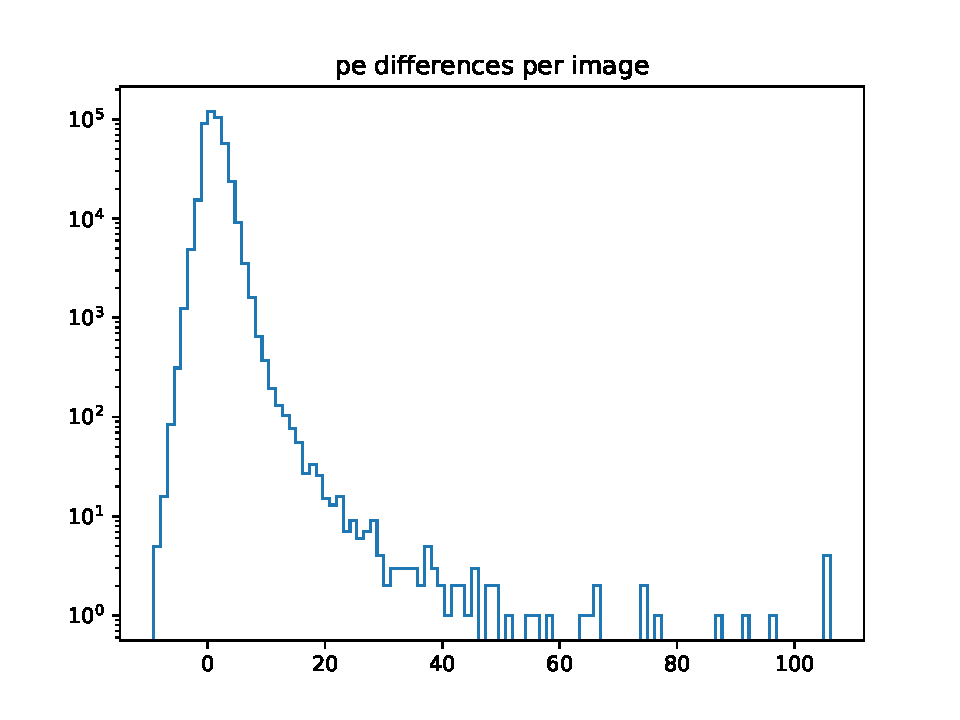
\includegraphics[width=0.5\textwidth]{Plots/diffs_hist_DBSCAN_pe_20131104_162_logy.pdf}
  }
  \subcaptionbox{Normalized distribution.\label{fig:pe_diffs}}[0.5\textwidth]{
    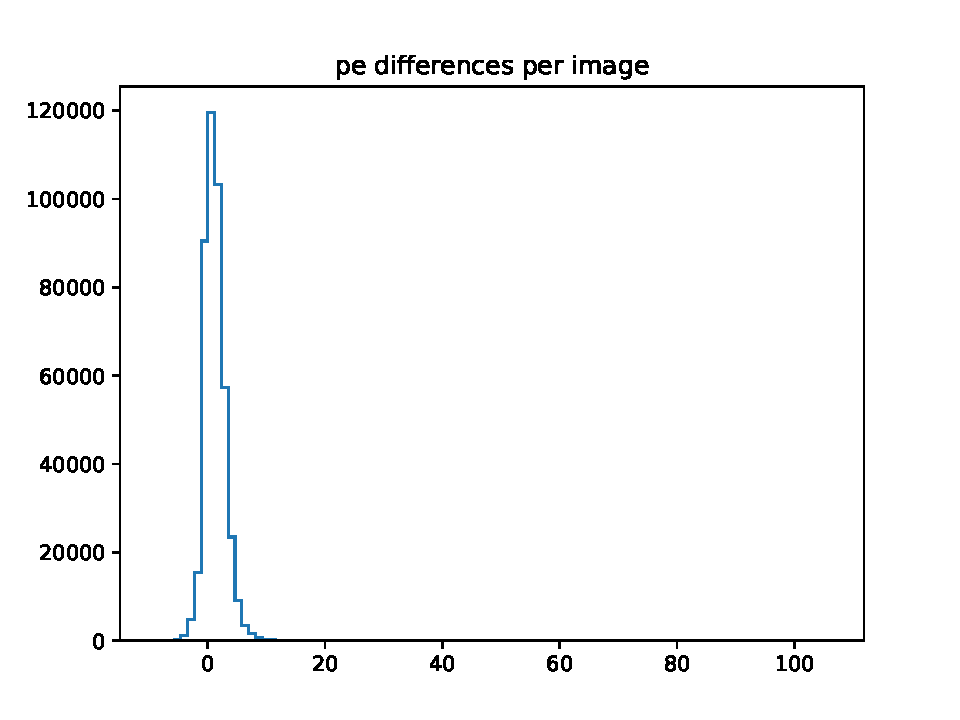
\includegraphics[width=0.5\textwidth]{Plots/diffs_hist_DBSCAN_pe_20131104_162.pdf}
  }
  \caption{PE differences per event and pixel between LP data and PhotonStream data accumulated for 300 events and normalized.}
  % \label{fig:pe_diffs}
\end{figure}
%

\autoref{fig:pe_diffs} shows the distribution of the PE differences as
described above accumulated for 300 events. The PhotonStream data on average contains
aorund 2 PE more than the corresponding LP event. However, as is visible in
\autoref{fig:pe_diffs_log} there is quite a number of pixels deviating by up to
20 PE. This reflects the observations from the four example events discussed
above: the majority of pixels contains one to two PE more than the PhotonStream
data while the few shower pixels contain a larger amount of PE more than the LP
data.


%
\begin{figure}
  \begin{subfigure}{0.5\textwidth}
    \centering
    \includegraphics[width=\textwidth, page=17]{Plots/pe_difference_pe_20131104_162.pdf}
  \end{subfigure}
  \begin{subfigure}{0.5\textwidth}
    \centering
    \includegraphics[width=\textwidth, page=26]{Plots/pe_difference_pe_20131104_162.pdf}
  \end{subfigure}
  \caption{PE differences between PhotonStream and LP data for two different events (32 and 51). The top camera image
  shows the PE as generated by the photon extractor for the PhotonStream. The
  bottom image shows the PE as generated from the LP of the time series. The
  middle image shows the difference of both images in PE per pixel.}
  \label{fig:difference}
\end{figure}
%
%
\begin{figure}
  \begin{subfigure}{0.5\textwidth}
    \centering
    \includegraphics[width=\textwidth, page=33]{Plots/pe_difference_pe_20131104_162.pdf}
  \end{subfigure}
  \begin{subfigure}{0.5\textwidth}
    \centering
    \includegraphics[width=\textwidth, page=53]{Plots/pe_difference_pe_20131104_162.pdf}
  \end{subfigure}
  \caption{PE differences between PhotonStream and LP data for two different events (67 and 111). The top camera image
  shows the PE as generated by the photon extractor for the PhotonStream. The
  bottom image shows the PE as generated from the LP of the time series. The
  middle image shows the difference of both images in PE per pixel.}
  \label{fig:difference2}
\end{figure}


%%%%%%%%%%%%%%%%%%%%%%%%%%%%%%%%%%%%%%%%%%%%%%%%%%%%%%%%%%%%%%%%%%%%%
\section{Standard Features on the PhotonStream}\label{sec:features_phs}
%%%%%%%%%%%%%%%%%%%%%%%%%%%%%%%%%%%%%%%%%%%%%%%%%%%%%%%%%%%%%%%%%%%%%
%
Using the single extracted photons from the PhotonStream, every classical
analysis parameter can be generated, because the photons can be accumulated
along their time axis to reproduce a camera image like the one from LP data. Of
course, the big opportunity of the PhotonStream is the additional timing
information per photon, which may yield new possibilities for analyses.
Nonetheless, it is neccessary to understand the differences on known territory
and thus to examine the classical features. For the general purpose of
parametrizing events and analysing them, an open python package called
\texttt{FeatureStream}~\cite{FeatureStream} has been developed alongside this work. It contains
functions for all the data preparation steps and already contains a large
fraction of the classical features, along with some PhotonStream-specific ones.

\begin{figure}
  \begin{subfigure}{0.5\textwidth}
    \centering
  \includegraphics[width=\textwidth, page=3]{Plots/std_phs_comparison_hist_same_DBSCAN_crab.pdf}
  \end{subfigure}
  \begin{subfigure}{0.5\textwidth}
    \centering
    \includegraphics[width=\textwidth, page=3]{Plots/std_phs_comparison_DBSCAN_crab.pdf}
  \end{subfigure}
  \caption{\texttt{size} of the air-shower for the same events on PhotonStream data and DBSCAN cleaning (blue) and on LP data and FACT-Tools cleaning (orange).}
  \label{fig:size_comp}
\end{figure}
%
When comparing the \texttt{size} of the same events in PhotonStream data and LP data (\autoref{fig:size_comp}),
the conclusions from \autoref{sec:ph_ex} are confirmed: As shown in
\autoref{sec:ph_ex}, the photon extraction is generally reconstructing more PE
than LP data, especially within air-shower pixels, therefore also leading to
larger air-shower clusters than the classical approach.

The main features from the Hillas parametrization are \texttt{width} and
\texttt{length} along with higher order statistical moments and the
air-shower's \texttt{size}. \autoref{fig:feat_comp} shows the Hillas features for the same events on PhotonStream data and DBSCAN cleaning (blue) and on LP data and FACT-Tools cleaning (orange).
%
\begin{figure}
  \begin{subfigure}{0.5\textwidth}
    \centering
    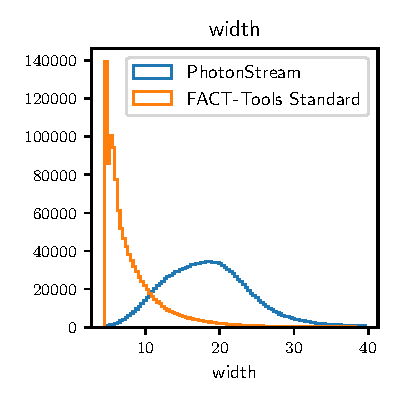
\includegraphics[width=\textwidth, page=1]{Plots/std_phs_comparison_hist_same_DBSCAN_crab.pdf}
  \end{subfigure}
  \begin{subfigure}{0.5\textwidth}
    \centering
    \includegraphics[width=\textwidth, page=2]{Plots/std_phs_comparison_hist_same_DBSCAN_crab.pdf}
  \end{subfigure}
  \begin{subfigure}{0.5\textwidth}
    \centering
    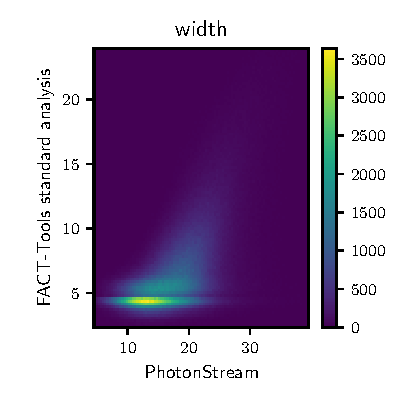
\includegraphics[width=\textwidth, page=1]{Plots/std_phs_comparison_DBSCAN_crab.pdf}
  \end{subfigure}
  \begin{subfigure}{0.5\textwidth}
    \centering
    \includegraphics[width=\textwidth, page=2]{Plots/std_phs_comparison_DBSCAN_crab.pdf}
  \end{subfigure}
  \caption{Hillas features for the same events on PhotonStream data and DBSCAN cleaning (blue) and on LP data and FACT-Tools cleaning (orange), as well as the twodimensional confusion matrix between the two analyses (bottom plots).}
  \label{fig:feat_comp}
\end{figure}
%
The direct comparison of the PhotonStream data's features illustrates the
differences of the cleaned air-showers: The air-shower's spatial features like
\texttt{width} and \texttt{length} are strongly shifted towards larger values.
From this it becomes clear that the DBSCAN cleaning is associating photons to
the shower cluster that lie within pixels far from the shower core, when
comparing to the classical cleaning. For the DBSCAN cleaning in the chosen
metric, photons that arrive in a close temporal proximity but within pixels not
containing large amounts of PE, can still easily be considered part of the
air-shower.

From these deviations another important question arises: how well do the MC
simulations describe the reality or in other words do simulations and data
match as expected? Without knowing which photons within an event are air-shower
photons and which not it is hard to tell, whether the different topology of the
PhotonStream clusters is closer to the real air-shower or not.
\textcolor{red}{[Untersuchungen von Sebastian?]} Independent from that it is crucial to
have that same behaviour on simulations. \autoref{fig:feat_dbscan} shows the
distributions of \texttt{width}, \texttt{length} and \texttt{size} of
PhotonStream data on the DBSCAN cleaning for data and the gamma and proton MC
simulations normalized to the respective observation time.

The vast majority of the observed data is generally expected to be proton
events or other background. Therefore, the distributions of data and proton MC
should be more or less similar. When comparing the distributions in
\autoref{fig:feat_dbscan} there seems to be a shift of the proton MC
simulations to slightly higher values for \texttt{width} and \texttt{length}.
So the air-shower clusters reconstructed on the proton MC simulations are
usually a bit bigger. Apart from that the distributions show a similar shape.
When comparing the \texttt{size} of the found air-showers, the data events
contain a lot more small-sized events than the simulated proton MC. This is
expected, because the data naturally contains a lot of noise and other rather
low energy events with small sizes. However, the distributions show very
similar structures on the whole range, even at the lower end. Spatially bigger
air-showers and bigger values for \texttt{size} in the MC simulations might
appear due to missing noise events in the simulations.

When expanding the DBSCAN clustering by excluding very dark pixels (containing less than $\SI{1}{\percent}$ of the shower's \texttt{size}) from the
calculations of \texttt{width} and \texttt{length},
\autoref{fig:feat_dbscan_perc}, the proton MC distributions of those features
are shifted to smaller values, as expected. The distributions of the features
on data are not really affected much, resulting in a better agreement of data
and MC simulations. The additional pixels, the DBSCAN is associating to the air-shower as compared to the standard cleaning seem to be one cause for the mismatches of simulations and observed data.
%
\begin{figure}
  \begin{subfigure}{0.5\textwidth}
    \centering
    \includegraphics[width=\textwidth, page=23]{Plots/data_mc/features_DBSCAN.pdf}
  \end{subfigure}
  \begin{subfigure}{0.5\textwidth}
    \centering
    \includegraphics[width=\textwidth, page=13]{Plots/data_mc/features_DBSCAN.pdf}
  \end{subfigure}
  \begin{subfigure}{0.5\textwidth}
    \centering
    \includegraphics[width=\textwidth, page=15]{Plots/data_mc/features_DBSCAN.pdf}
  \end{subfigure}
  \begin{subfigure}{0.5\textwidth}
    \centering
    \includegraphics[width=\textwidth, page=8]{Plots/data_mc/features_DBSCAN.pdf}
  \end{subfigure}
  \caption{Features of the reconstructed air-showers using the DBSCAN cleaning. The blue histograms show the observed data, whereas orange and green show proton and gamma MC simulations respectively. The histograms are normalized to the respective observation time or simulated observation time.}
  \label{fig:feat_dbscan}
\end{figure}
%
%
\begin{figure}
  \begin{subfigure}{0.5\textwidth}
    \includegraphics[width=\textwidth, page=23]{Plots/data_mc/features_DBSCAN_perc.pdf}
  \end{subfigure}
  \begin{subfigure}{0.5\textwidth}
    \includegraphics[width=\textwidth, page=13]{Plots/data_mc/features_DBSCAN_perc.pdf}
  \end{subfigure}
  \caption{Features of the reconstructed air-showers using DBSCAN and additionally excluding pixels with less than $\SI{1}{\percent}$ PE of the air-shower's total \texttt{size}. The blue histograms show the observed data, whereas orange and green show proton and gamma MC simulations respectively. The histograms are normalized to the respective observation time or simulated observation time.}
  \label{fig:feat_dbscan_perc}
\end{figure}
%
From the feature distributions it becomes clear that there are regions, where
data and MC simulations fit better. The \texttt{size} is in better agreement
above a threshold of about \num{100}. In general, events with a big size are
less prone to reconstruction errors, since  noise fluctuations in the number of
PE and in the spatial distribution of photons, both affecting the origin
reconstruction, are suppressed. Small clusters, especially within the data
might very well also be noise events. However, they appear in data, but are not
accounted for in the MC simulations used for training the random forests, making them a likely source of error.

Especially with respect to the origin reconstruction, the number of pixels
\texttt{n\_pixel} associated with an air-shower is important for the accuracy
of the reconstructed position. Very small events are strongly influenced by
fluctuating neighboring pixels and the main axis direction is generally hard to
reconstruct. Due to the quantization of the single pixels a singular photon
within a neighboring pixel can impact the result significantly.
The optimization of the cuts on all used features has to be performed in
detail beyond the scope of this thesis, but to investigate the potential of the
PhotonStream data, the quality cuts are restrained to those excluding events,
which are intrinsically prone to reconstruction errors.

%%%%%%%%%%%%%%%%%%%%%%%%%%%%%%%%%%%%%%%%%%%%%%%%%%%%%%%%%%%%%%%%%%%%%
\section{Time Features on the PhotonStream}
%%%%%%%%%%%%%%%%%%%%%%%%%%%%%%%%%%%%%%%%%%%%%%%%%%%%%%%%%%%%%%%%%%%%%
%
The PhotonStream does not only open the possibilities for analyses of single
photon features, while still containing all relevant data from the classical
representation, it furthermore contains \textbf{time information} per photon.
This additional dimension in the data makes it even more interesting for
analyses and might promise great advances in performance.

With the additional time information a series of new features can be
implemented. The classical features can be expanded onto this dimension,
examining the light distributions along the time axis and calculating
statistical moments of them. There are additional angles describing the
shower's position when working in three dimensions, and new features can be
engineered. These new features possibly offer a way to strongly boost
performance by taking advantage of the new additional dimension.

The distributions of arrival times of the single photons for data and MC
simulations are shown in \autoref{fig:slices}. The histograms show the arrival
times for every single photon of 2000 events normalized to an area of 1. The
top histogram represents all arriving photons. It becomes clear that there
seems to be a significant discrepancy between the MC simulations and data.
While distributions of the MC simulations of both, gammas and protons, quite
resemble each other, the data distribution shows a very different picture. The
most common arrival time of data lies way beyond the one on MC simulations.
Furthermore, the structure of the distribution before the main peak in data
shows two dips and generally not a very clear distribution as compared to the
monotonous rise of the MC distributions. This behaviour might result from noise
events and falsely triggered events or originate from electronic artifacts. To
investigate the origins of this structure, the bottom histogram shows the
arrival times of all photons located in pixels with at least \num{10} photons.
This way the fraction of non air-shower photons becomes very small. In the
result the normally distributed underground, as seen in the top histogram,
vanishes almost completely. The most common arrival times for the MC
simulations become sharper but remain at the same position as before. In
contrast to the complete events, the data distribution now shows a peak near
the ones in the MC simulations and does no longer show the unstructered
behaviour in the first \num{40} time slices as described above. The difference
between data and MC simulations still manifests between time slices \num{60}
and \num{80}, though. The data distribution decreases slower and takes about
\num{20} time slices more to return to a supposed background level.
%
\begin{figure}
  \begin{subfigure}{\textwidth}
    \centering
    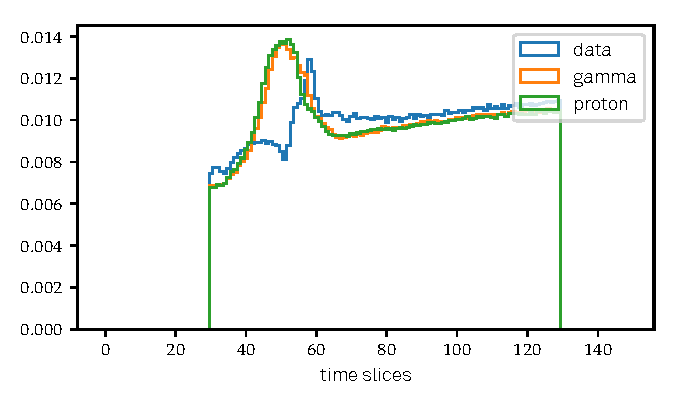
\includegraphics[width=0.8\textwidth]{Plots/all_slices_min_0_per_pixel.pdf}
  \end{subfigure}
  \begin{subfigure}{\textwidth}
    \centering
    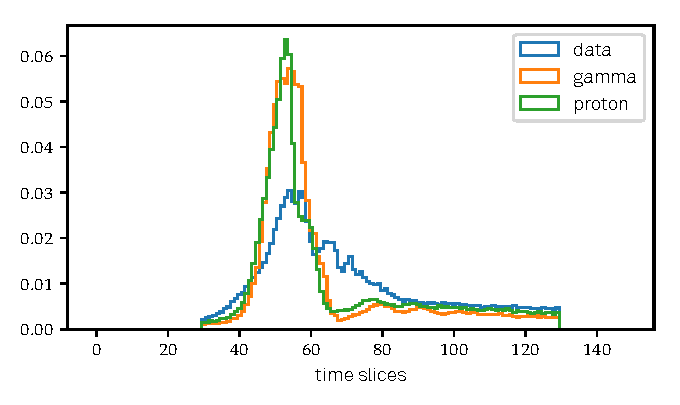
\includegraphics[width=0.8\textwidth]{Plots/all_slices_min_10_per_pixel.pdf}
  \end{subfigure}
  \caption{Arrival times of the single photons within all the pixels (top) and the cleaned air-shower pixels containing at least 10 photons (bottom) on data and MC simulations.}
  \label{fig:slices}
\end{figure}
%

The arrival time distributions show quite some disagreement in uncleaned
pixels, originating from data-MC-mismatches probably due to noise effects. For
the cleaned images, which are the crucial ones, the agreement is better, so
implementing time features into a working PhotonStream analysis is a natural
next step. Nonetheless, the mismatches need to be understood and potentially
improved, to get usefull features.

%%%%%%%%%%%%%%%%%%%%%%%%%%%%%%%%%%%%%%%%%%%%%%%%%%%%%%%%%%%%%%%%%%%%%
\section{Reconstruction of the Source Position}
%%%%%%%%%%%%%%%%%%%%%%%%%%%%%%%%%%%%%%%%%%%%%%%%%%%%%%%%%%%%%%%%%%%%%
%
As described in \autoref{sec:source_pos} the reconstruction of the source
position uses the air-shower's features \texttt{delta}, \texttt{width} and
\texttt{length}. The calculated angle \texttt{delta} plays a major role in
finding the right source position, since it describes the axis along which
the source position is assumed to be. It is calculated as the angle between
the shower's main axis and the camera's $x$-axis. Therefore, it is dependent
on the covariance of the light distribution and thus affected by the
differences within the PhotonStream.

To investigate the differences on PhotonStream data, it is possible to
calculate a true delta on the data images by using the telescope's pointing
position. From the pointing position and the known source position an
expected source position within the camera can be calculated. The
air-shower's \texttt{cog} and the calculated source position within the camera can
then be used to calculate a vector representing the estimated shower axis.
The calculated angle $\delta_\text{true}$ of that shower axis can thus be
compared to the calculated angle of the cleaned air-shower's main axis. The
distribution of these differences $\symup{\Delta}\delta$ is expected to have two peaks: one around
zero and one around a difference of $\pi$. These two peaks correspond to
air-showers with a very small difference in $\delta$ and on the one hand the
right estimated sign of \texttt{disp} (zero) and on the other hand the
opposite estimated sign of \texttt{disp} ($\pi$). When dividing the
distribution into the different signs of \texttt{disp} there should only be
one peak for each distribution for a working sign classifier.

\autoref{fig:delta_fact} shows a distribution of $\symup{\Delta}\delta$ for
the pixel based cleaning as described in \autoref{sec:thresh} on LP data.
The two histograms represent the different estimations of the sign of
\texttt{disp} for the whole open data sample. The distributions show very
good agreement with the expectations described above. While this is not a
comparison with any real truth, it nevertheless shows a working
reconstruction of the air-shower events.
%
\begin{figure}
  \centering
  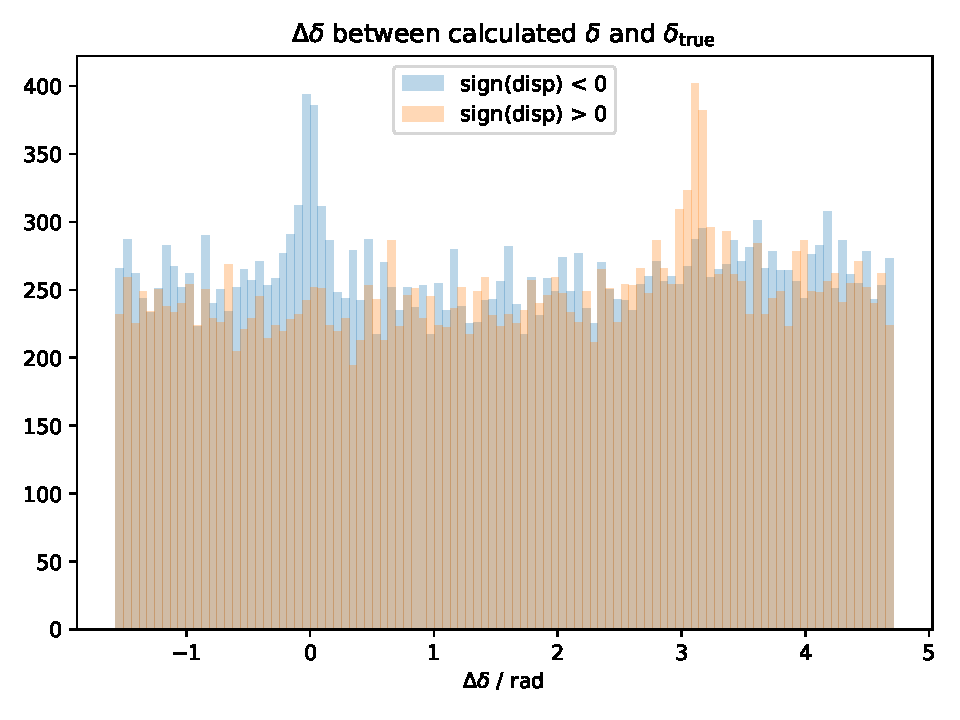
\includegraphics[width=0.7\textwidth]{Plots/delta_delta/delta_delta_facttools.pdf}
  \caption{Difference between calculated \texttt{delta} and true \texttt{delta} for the FACT-Tools analysis \cite{openana}. The distributions show the calculated $\symup{\Delta}\delta$ for the different predictions of sign of \texttt{disp} on the whole open data crab sample.}
  \label{fig:delta_fact}
\end{figure}
%
When calculating $\symup{\Delta}\delta$ on the cleaned PhotonStream data, a
very different picture emerges. \autoref{fig:delta_diff_a} shows
$\symup{\Delta}\delta$ for the DBSCAN cleaning, when projecting the found
photons back to the camera plane and calculating \texttt{delta}. There are
hardly any peaks in these distributions, but rather widely spread
accumulation ranges around zero and $\pi$. Thus, the calculated
\texttt{delta} seems to differ quite significantly from the expected
\texttt{delta}. Furthermore, both \texttt{sign} predictions show similar
distributions, hinting at a low accuracy for the \texttt{sign}
classification. The main difference between the air-showers found by DBSCAN
and the ones found by the classic cleaning projected to the camera plane is
the spread across the camera axes. DBSCAN clustering is associating photons
from pixels quite distant from the shower core to the air-shower cluster.
This way, the spread within $x$ and $y$ becomes way bigger. Because
\texttt{delta} is calculated on the $x$-$y$-distribution weighted by the
number of photons, these outlier photons might have a big impact on the
calculation of \texttt{delta}, even though they usually only contain very
few photons. To prevent this from happening, the cleaning can be extended by
a step excluding pixels with less than $\SI{1}{\percent}$ of the total
amount of photons from the calculations of \texttt{delta}, \texttt{length}
and \texttt{width}, as done for the feature distributions in \autoref{sec:features_phs}. The distributions of $\symup{\Delta}\delta$ for this
cleaning are shown in \autoref{fig:delta_diff_perc}.

\begin{figure}
  \subcaptionbox{\label{fig:delta_diff_a}}[0.48\textwidth]{
    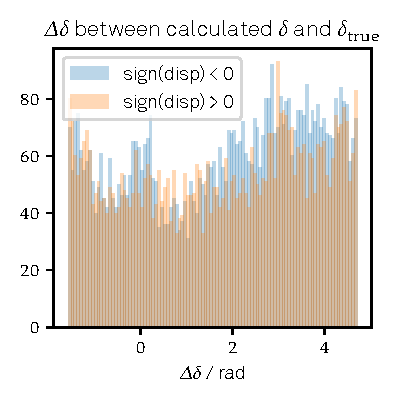
\includegraphics[width=0.5\textwidth]{Plots/delta_delta/delta_true_diff_hist_thresholds_rad_20131104_162.pdf}
  }
  \subcaptionbox{\label{fig:delta_diff_perc}}[0.48\textwidth]{
    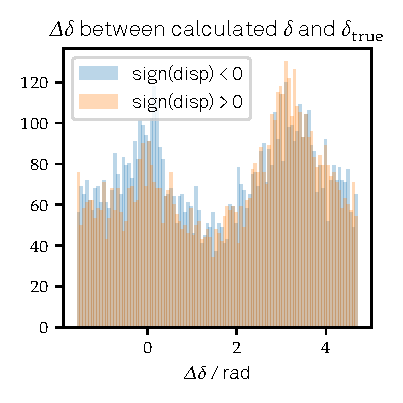
\includegraphics[width=0.5\textwidth]{Plots/delta_delta/delta_delta _DBSCAN_1perc_rad_20131104_162.pdf}
  }
  \caption{Difference between calculated delta and true delta for a subset of 500 data events. delta is calculated using all cleaned pixels \protect\subref{fig:delta_diff_a} and using only cleaned pixels containing more than $\SI{1}{\percent}$ of the air-shower's size \protect\subref{fig:delta_diff_perc}.}
  \label{fig:true_delta}
\end{figure}
%
The distributions change significantly, when adapting the cleaning.
The two peaks become quite distinctive around $0$ and $\pi$. Also the
different \texttt{sign} predictions show different heights around the two
accumulation points corresponding to the rightly classified signs, although
there seem to be frequent misclassifications. Although the results still
differ strongly from the ones shown in \autoref{fig:delta_fact}, the
accuracy of the reconstructed \texttt{delta} improves when neglecting outlying pixels. Thus, there
seems to be an impact of the large spread of DBSCAN clusters which is very
likely to also affect the origin reconstruction on such events. This mismatches
therefore might be reduced when adapting the metric of the three-dimensional
spacetime of the point cloud.

%
\begin{figure}
  \centering
  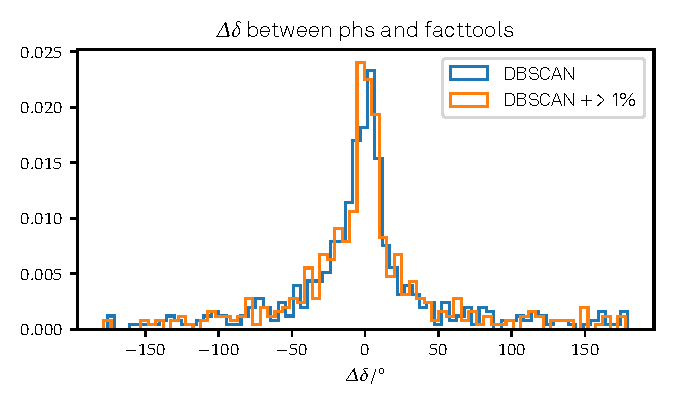
\includegraphics[width=\textwidth]{Plots/delta_delta/delta_diff_hist_perc_and_normal_DBSCAN_delta_20131104_162.pdf}
  \caption{Differences between the PhotonStream \texttt{delta} and the FACT-Tools \texttt{delta} for the DBSCAN cleaning (blue) and the DBSCAN cleaning extended by excluding pixels with less than $\SI{1}{\percent}$ of the shower's \texttt{size} (orange).}
  \label{fig:delta}
\end{figure}
%
Since the FACT-Tools analysis yields good results and a working origin
reconstruction, the differences between its features and the DBSCAN cluster
features can also be investigated to understand the new data representation.
\autoref{fig:delta} shows the differences between the PhotonStream
\texttt{delta} and the FACT-Tools \texttt{delta} for the DBSCAN cleaning (blue
histogram) and the DBSCAN cleaning extended by excluding pixels with less
than $\SI{1}{\percent}$ of the shower's \texttt{size} (orange histogram).
From these distributions, it becomes clear that the difference of the
PhotonStream's air-showers does not solely result from the wider spread of
the light distribution over the camera pixels. The two distributions barely
differ from another, although as shown by \autoref{fig:delta_diff_perc}, the
reconstruction of \texttt{delta} seems to improve with the additional
cleaning. For the majority of events the calculated \texttt{delta} is within
$\mathcal{O}(\SI{10}{\degree})$ to the FACT-Tools \texttt{delta}, but for the
origin reconstruction such a difference can become a difficult obstacle.
However, this comparison, as the one with the expected source position
within the camera, is not a comparison with truth values, but rather one
with a working analysis.

%%%%%%%%%%%%%%%%%%%%%%%%%%%%%%%%%%%%%%%%%%%%%%%%%%%%%%%%%%%%%%%%%%%%%
\subsection{Reconstruction of the Source Position on Data}
%%%%%%%%%%%%%%%%%%%%%%%%%%%%%%%%%%%%%%%%%%%%%%%%%%%%%%%%%%%%%%%%%%%%%

All these investigations, of course, serve the sole purpose of understanding
the different prerequisites for reconstructing the source position on
air-shower images. As described in \autoref{sec:source_pos} this is done by
using the disp-method on Hillas parametrized images. Random forests
are used to estimate $|\texttt{disp}|$ via a regression task and then determine
the $\text{sign}(\texttt{disp})$ via a classification. The used random forests
consist of \num{100} estimators, each of which has a maximum depth of \num{15} and $\sqrt{N}$ of $N$ total features available at each node.

The output of these random forests can then be projected from the air-shower's
core within the camera to sky coordinates, resembling the estimated source
position. Since the Crab Nebula is a well known source with a well known
position, the difference between the reconstructed and the known source
position can be calculated. It is tipically quantized as the euklidian distance
squared in $[\theta^2] = \si{\degree\squared}$ and illustrated as shown in
\autoref{fig:theta2}. These $\theta^2$-plots show the distribution of the
distances squared of the reconstructed source position per event from the Crab
Nebula's known position. They contain all events after preselection cuts and
applying the gamma hadron separation at a specific \texttt{gamma\_prediction}
threshold. The blue bins show the reconstructed signal events (On events) when
pointing directly to the source position while the orange bins represent the
reconstructed background events (Off events), pointing to the night sky next to
the source. The $\theta^2$-cut, represented by the dashed, grey vertical line,
represents the optimal cut for the source's detection significance on signal events. Events between $\theta^2 = 0$ and this cut are considered when calculating the excess significance.
The ratio of on-source observation time and off-source observation time is
$\alpha = 0.2$. This fraction is used to estimate the background within the
on-source observations. Both, $\theta^2$-cut and the \texttt{gamma\_prediction}
threshold are determined by finding the highest significance, calculated as
described by Li \& Ma \cite{LiMa}.

The used random forest is trained on gamma and proton MC simulations to perform
the \texttt{disp} regression and the \texttt{sign} classification. The
performance results of this training are very good for the \texttt{sign}
classification, while the regression of \texttt{disp} seems to be more
difficult. The accuracy of the \texttt{sign} classification averaged from the
cross-validation is $0.7923\,\pm\,0.0018$. Slightly outperforming the FACT-
Tools analysis with an accuracy of $0.7537\,\pm\,0.0018$. The regression of
\texttt{disp}, however, only reaches an $R^2$ score of $0.5385\,\pm\,0.0046$,
which is quite low and might strongly affect the accuracy of the origin
reconstruction. The FACT-Tools analysis, in comparison, reaches an $R^2$ score
of $0.6631\,\pm\,0.0044$.

For a Crab Nebula data sample and a working analysis the $\theta^2$-plot is
expected to have an equally distributed, low number of Off-events with a
significant excess of On-events as close to $\theta^2 = 0$ as possible. From
the results shown in \autoref{fig:theta2} it becomes very clear, that the
reconstruction of the PhotonStream data in the way described above does not
yield a very good source reconstruction on data. The optimal $\theta^2$-cuts
around \num{0.1} are quite large. The distribution of the On-events around the
true source position are rather fuzzy: there is no clear peak, especially not
around \num{0}. The source excess starts around \num{0.10} and grows until
between \num{0} and \num{0.05}. Thus, the reconstruction of the source position
and especially the regression of \texttt{disp} seem to have a big error margin,
reconstructing events to the close proximity of the true source position. Since
$\theta$ is not the error on the reconstructed position, but rather the
distance of all cleaned events to a specific source, the cleaning and
especially the gamma hadron separation affect the results just as much.
%
\begin{figure}
  \begin{subfigure}{\textwidth}
    \centering
    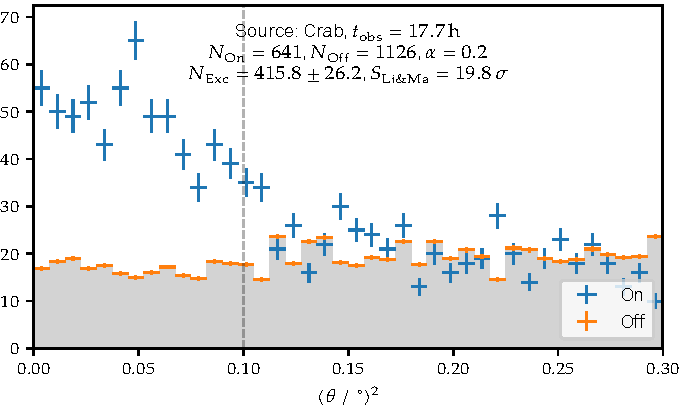
\includegraphics[width=\textwidth]{Plots/results/DBSCAN/theta2_plot.pdf}
  \end{subfigure}
  \begin{subfigure}{\textwidth}
    \centering
    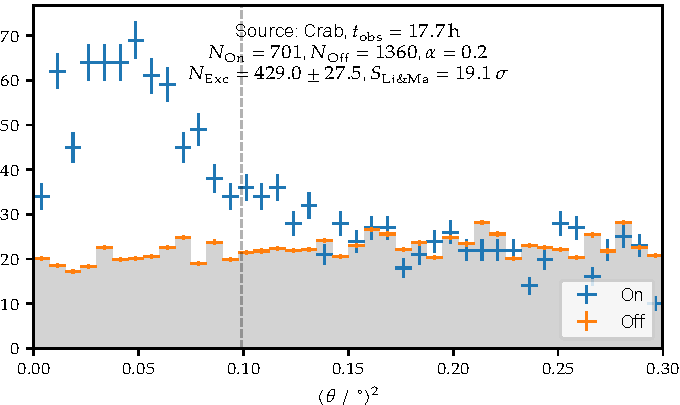
\includegraphics[width=\textwidth]{Plots/results/DBSCAN_perc/theta2_plot.pdf}
  \end{subfigure}
  \caption{$\theta^2$-plots for the PhotonStream data and dedicated analysis for the DBSCAN cleaning (top) and extended by excluding pixels with less than $\SI{1}{\percent}$ of the air-shower's \texttt{size} (bottom), to test the better data-MC agreement of that cleaning. They contain all events after preselection cuts and applying the gamma hadron separation at a specific \texttt{gamma\_prediction} threshold. The blue bins show the reconstructed signal events (On events) when pointing directly to the source position while the orange bins represent the reconstructed background events (Off events), pointing to the night sky next to the source.}
  \label{fig:theta2}
\end{figure}
%

%%%%%%%%%%%%%%%%%%%%%%%%%%%%%%%%%%%%%%%%%%%%%%%%%%%%%%%%%%%%%%%%%%%%%
\section{Gamma Hadron Separation}
%%%%%%%%%%%%%%%%%%%%%%%%%%%%%%%%%%%%%%%%%%%%%%%%%%%%%%%%%%%%%%%%%%%%%
%
The observed data mainly consists of proton events, since the majority of the
cosmic ray flux consists of protons. Therefore, it is important to distinguish
gamma air-shower events from proton events, which are considered background for
this analysis. A working gamma hadron separation affects all steps of the
analysis, because the energy reconstruction is trained on gamma events as well
as the source reconstruction. A badly cleaned data set thus will not work well
with the trained models.

For this analysis a random forest is used for the classification. It consists
of \num{100} estimators, each of which has a maximum depth of \num{15} and $\sqrt{N}$ of $N$ total features available at each node. The forest is trained on the features shown in \autoref{fig:sep_feat}.
This figure also shows the proportional importances of the single features
within the trained model. The most important features for the separation are
the \texttt{width} and \texttt{kurtosis\_trans}, the higher order statistical
moment along the same axis. From this, one can see that the spatial topology of
the air-shower is the main discriminator.

% neccessary line ^^^^
\begin{figure}
  \centering
  \includegraphics[width=0.8\textwidth, page=4]{Plots/results/DBSCAN/separation_performance.pdf}
  \caption{Features used for the gamma hadron separation model. The features are defined in \autoref{sec:params} and sorted by their importance for the separation task.}
  \label{fig:sep_feat}
\end{figure}
%
The trained model can be validated on the MC data, because the particle type is
known for the datasets. To do so, the model is trained on a subset of the
available simulations to then be validated on the small complementary
dataset. To avoid statistical fluctuations within the subsamples to affect the
results, a cross-validation is used. \autoref{fig:sep_auc} shows the ROC curve
of the trained model, consisting of the true positive rate as a function of the
false positive rate. The blue line shows the results of the averaging from the
cross-validation. The AUC is $0.8425\,\pm\,0.0016$ with the error resulting
from the averaging. This is a very good result for the separation of the gamma
showers from the proton background, especially since this analysis is not
primarily focused on optimizing these metrics. However, this is a result on
Monte Carlo simulations and the quality of the model on data might differ quite
significantly.
%
\begin{figure}
  \centering
  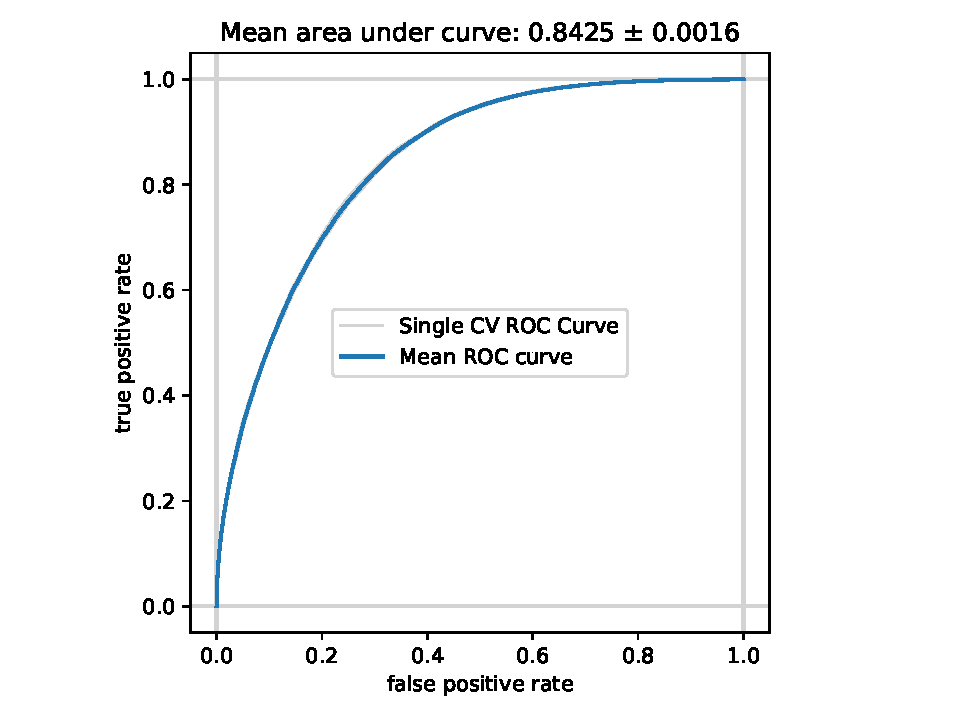
\includegraphics[width=0.8\textwidth, page=1]{Plots/results/DBSCAN/separation_performance.pdf}
  \caption{\textit{Receiver Operating Characteristic} (ROC) curve for the binary gamma hadron separation. The true positive rate as a function of the false positive rate is shown in grey. The blue line represents the averaged result out of a 5-fold cross-validation. The averaged \textit{area under curve} (AUC) from the 5-fold cross-validation for the trained models is $0.8425\,\pm\,0.0016$ with the error resulting from the averaging.}
  \label{fig:sep_auc}
\end{figure}
%
%
% \begin{figure}
%   \centering
%   \includegraphics[width=0.8\textwidth, page=3]{Plots/results/DBSCAN/separation_performance.pdf}
%   \caption{Gamma hadron separation plot.}
%   \label{fig:sep2}
% \end{figure}
%
%%%%%%%%%%%%%%%%%%%%%%%%%%%%%%%%%%%%%%%%%%%%%%%%%%%%%%%%%%%%%%%%%%%%%
\section{Energy Estimation}
%%%%%%%%%%%%%%%%%%%%%%%%%%%%%%%%%%%%%%%%%%%%%%%%%%%%%%%%%%%%%%%%%%%%%
%
The reconstruction of the air-shower's energy is applied on cleaned and as
gamma air-shower classified images. It uses the same features as the separation
model. Since the PhotonStream paired with DBSCAN reconstructs bigger air-shower
images and a larger number of photons it is interesting to investigate the
results on the reconstructed energy.

For this analysis a random forest is used for the energy estimation, as well.
It performs a regression task and consists of \num{100} decision trees and a
maximum depth of \num{15} for the single tree. The forest is trained on the
features shown in \autoref{fig:energy_feat}. In addition to the features described in \autoref{sec:params}, the \texttt{area} of the shower is used for the energy estimation. It is defined as
%
\begin{equation}
  \texttt{area} = \texttt{width}\times\texttt{length}\times\symup{\pi}\, .
\end{equation}
%
\autoref{fig:energy_feat} also shows the
proportional importances of the single features within the trained model. The
most important features for the energy estimation of a shower are those
strongly correlated with the number of photons within the air-shower. The
\texttt{size} and the number of pixels associated with the air-shower
(\texttt{n\_pixel}) are by far the most important features, together making up
almost $\sfrac{2}{3}$ of the total importance. Of course, since the number of
photons depends on the number and energy of secondary particles, which itself
depends on the energy of the primary particle, one would expect that.
%
\begin{figure}
  \centering
  \includegraphics[width=0.9\textwidth, page=4]{Plots/results/DBSCAN/energy_performance.pdf}
  \caption{Features used for the energy estimation model. The features are defined in \autoref{sec:params} and sorted by their importance for the estimation task.}
  \label{fig:energy_feat}
\end{figure}
%

Since the primary particle's energy an air-shower was simulated with is known
for the simulation data, the performance of the trained model can be
validated on the MC simulations. \autoref{fig:energy_matr} shows the confusion
matrix for the energy estimation. The energy estimated by the random forest
($y$-axis) is shown against the event's true energy ($x$-axis). A clear
correlation is visible on the diagonal, showing that the trained model is
reconstructing energies close to the true energies. Rather than a thin line,
the spread of this distribution however is quite wide. The reconstructed
energies therefore lie within a wide error margin around the true energy.
Especially for low energies the spread becomes very large. Air-showers
resulting from low energy primary particles contain less Cherenkov photons, as
described above. Therefore the reconstructed air-shower not only contains less
photons but also illuminates a smaller area of the camera. Thus, fluctuations
become more important and the accurate reconstruction of the image features more
difficult. Low energy events consequently are intrinsically harder to assign
the right energy to.
%
\begin{figure}
  \centering
  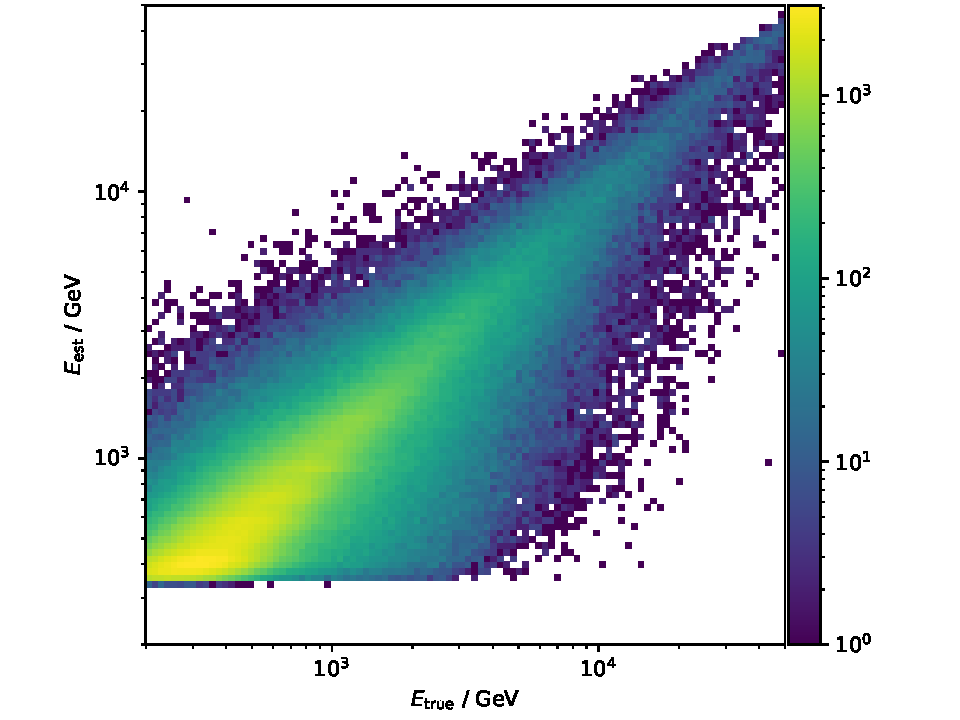
\includegraphics[width=0.9\textwidth]{Plots/results/DBSCAN/energy_migration.pdf}
  \caption{Confusion matrix for the estimation of the primary particle's energy. The energy estimated by the random forest ($y$-axis) is shown against the event's true energy ($x$-axis).}
  \label{fig:energy_matr}
\end{figure}
%
The resulting $R^2$ score for the best energy estimation model on PhotonStream
data is $R^2 = 0.74$. This is a quite good score for the energy estimation and
shows that the energy reconstruction works well on the gamma MC simulations.
Especially when compared to the FACT-Tools open data analysis~\cite{openana},
which reaches an $R^2$ score of $0.6876$, this result outperforms the
classical analysis.
%
% The energy bias and resolution of the analysis are shown for bins of true gamma
% energy in \autoref{fig:bias}.
% %
% \begin{figure}
%   \centering
%   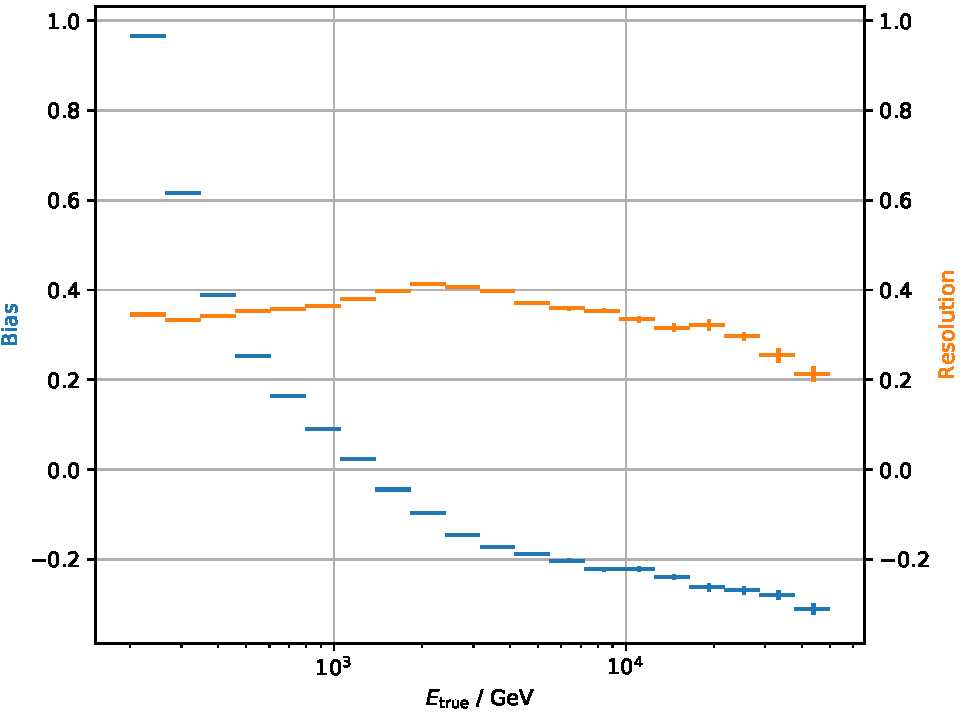
\includegraphics[width=0.9\textwidth]{Plots/results/DBSCAN/bias_resolution.pdf}
%   \caption{Bias (blue histogram) and resolution (orange histogram) of the PhotonStream data on DBSCAN cleaning as a function of true Energy of the gamma rays.}
%   \label{fig:bias}
% \end{figure}
% %


%%%%%%%%%%%%%%%%%%%%%%%%%%%%%%%%%%%%%%%%%%%%%%%%%%%%%%%%%%%%%%%%%%%%%
\section{Parameters of DBSCAN}
%%%%%%%%%%%%%%%%%%%%%%%%%%%%%%%%%%%%%%%%%%%%%%%%%%%%%%%%%%%%%%%%%%%%%
%
The physical properties used for this analysis are derived from the cleaned
images, i.e. the reconstructed shower clusters. The reconstruction of these
clusters is done by the DBSCAN algorithm. To set the right topology for the
clustering, DBSCAN is defined by two dedicated parameters, as described in
\autoref{sec:phs_clean}. The used parameters can be optimized for the analysis,
as well. However, there does not appear to be reason to believe that an
analysis specific set of the two parameters needs to be derived.

The minimum number of photons within a cluster $m$ has not been investigated. A
minimum number of \num{20} photons excludes only very small noise clusters. For
the analysis, the cuts in \texttt{size} and \texttt{n\_cluster} will then
exclude the small events.

The minimum distance $\varepsilon$ for a photon to still be associated with a
dense cluster has been investigated to be \num{0.1} for optimal results. The
effects of this parameter on the features of the air-shower clusters can be
examined nonetheless. \autoref{fig:eps_feat1}, \ref{fig:eps_feat2} and
\ref{fig:eps_feat3} show the distributions of the number of reconstructed
clusters and the spatial dimension of the air-shower represented by the
\texttt{width} for clusterings with different $\varepsilon$-configurations. To
give a picture of the dependance $\varepsilon$ is varied below and above the
default value of \num{0.1}. To simultaneously give a hint on the agreement of
MC simulations and the observed data, the proton MC simulated data (orange) is
also shown. The distributions are normalized to their observation time and the
expected night sky flux.

The effect of $\varepsilon$ on the topology of the clusters becomes very clear
when comparing the feature distributions for different values of $\varepsilon$.
The bigger $\varepsilon$ is set, the bigger the \texttt{width} gets. Therefore,
going to smaller values, the air-shower clusters will be confined to a smaller
space. The number of reconstructed clusters also gradually rises when setting
a bigger $\varepsilon$. This is to be expected, since a bigger $\varepsilon$
allows for less dense regions of the point cloud to be considered a dense
cluster. At some point this will lead to noise or ambient light to be
classified as air-shower clusters. For $\varepsilon = 0.11 / 0.12$ however, it
definiteley leads to large mismatches between MC simulations and data, that
become very clear for $\varepsilon = 0.14$. For $\varepsilon = 0.175$ the
distance for photons within a cluster becomes so big, that the initial large
number of small clusters decreases again, because many of these are combined to
a few bigger clusters.

For the observed data another development for bigger values of $\varepsilon$
emerges: The number of found air-showers within data events compared to those
found in proton MC simulations rises. This supposedly is the result of the
clustering reconstructing noise events within the data, that are not present in
the proton MC simulations. All in all, the agreement of simulations and data
seem to be best for smaller $\varepsilon$, rather than ones above \num{0.1}.

%
\begin{figure}
  \begin{subfigure}{0.5\textwidth}
    \centering
    $\symbf{\varepsilon = 0.07}$\par\smallskip
    \includegraphics[width=0.9\textwidth, page=23]{Plots/Epsilon/07_comparison.pdf}
  \end{subfigure}
  \begin{subfigure}{0.5\textwidth}
    \centering
    $\symbf{\varepsilon = 0.07}$\par\smallskip
    \includegraphics[width=0.9\textwidth, page=2]{Plots/Epsilon/07_comparison.pdf}
  \end{subfigure}
%%%%%%%%%%%%%%%%%%%%%%%%%%%%%%%%%%%%%%%%%%%%%%%%%%%%
  \begin{subfigure}{0.5\textwidth}
    \centering
    $\symbf{\varepsilon = 0.09}$\par\smallskip
    \includegraphics[width=0.9\textwidth, page=23]{Plots/Epsilon/09_comparison.pdf}
  \end{subfigure}
  \begin{subfigure}{0.5\textwidth}
    \centering
    $\symbf{\varepsilon = 0.09}$\par\smallskip
    \includegraphics[width=0.9\textwidth, page=2]{Plots/Epsilon/09_comparison.pdf}
  \end{subfigure}
  %%%%%%%%%%%%%%%%%%%%%%%%%%%%%%%%%%%%%%%%%%%%%%%%%%%%
  \caption{Distributions of the number of reconstructed
  clusters and the spatial dimension of the air-shower represented by the
  \texttt{width} for clusterings with different $\varepsilon$-configurations. To simultaneously give a hint on the agreement of MC simulations and the observed data, the proton MC simulated data (orange) is also shown. The distributions are normalized to their observation time and the expected night sky flux. The default value is $\varepsilon = 0.1$.}
  \label{fig:eps_feat1}
\end{figure}
%
%
\begin{figure}
  \begin{subfigure}{0.5\textwidth}
    \centering
    $\symbf{\varepsilon = 0.10}$\par\smallskip
    \includegraphics[width=0.9\textwidth, page=23]{Plots/Epsilon/10_comparison.pdf}
  \end{subfigure}
  \begin{subfigure}{0.5\textwidth}
    \centering
    $\symbf{\varepsilon = 0.10}$\par\smallskip
    \includegraphics[width=0.9\textwidth, page=2]{Plots/Epsilon/11_comparison.pdf}
  \end{subfigure}
  %%%%%%%%%%%%%%%%%%%%%%%%%%%%%%%%%%%%%%%%%%%%%%%%%%%%
  \begin{subfigure}{0.5\textwidth}
    \centering
    $\symbf{\varepsilon = 0.12}$\par\smallskip
    \includegraphics[width=0.9\textwidth, page=23]{Plots/Epsilon/12_comparison.pdf}
  \end{subfigure}
  \begin{subfigure}{0.5\textwidth}
    \centering
    $\symbf{\varepsilon = 0.12}$\par\smallskip
    \includegraphics[width=0.9\textwidth, page=2]{Plots/Epsilon/12_comparison.pdf}
  \end{subfigure}
  %%%%%%%%%%%%%%%%%%%%%%%%%%%%%%%%%%%%%%%%%%%%%%%%%%%%
  \caption{Distributions of the number of reconstructed
  clusters and the spatial dimension of the air-shower represented by the
  \texttt{width} for clusterings with different $\varepsilon$-configurations. To simultaneously give a hint on the agreement of MC simulations and the observed data, the proton MC simulated data (orange) is also shown. The distributions are normalized to their observation time and the expected night sky flux. The default value is $\varepsilon = 0.1$.}
  \label{fig:eps_feat2}
\end{figure}
%
%
\begin{figure}
  \begin{subfigure}{0.5\textwidth}
    \centering
    $\symbf{\varepsilon = 0.14}$\par\smallskip
    \includegraphics[width=0.9\textwidth, page=23]{Plots/Epsilon/14_comparison.pdf}
  \end{subfigure}
  \begin{subfigure}{0.5\textwidth}
    \centering
    $\symbf{\varepsilon = 0.14}$\par\smallskip
    \includegraphics[width=0.9\textwidth, page=2]{Plots/Epsilon/14_comparison.pdf}
  \end{subfigure}
  %%%%%%%%%%%%%%%%%%%%%%%%%%%%%%%%%%%%%%%%%%%%%%%%%%%%
  \begin{subfigure}{0.5\textwidth}
    \centering
    $\symbf{\varepsilon = 0.175}$\par\smallskip
    \includegraphics[width=0.9\textwidth, page=22]{Plots/Epsilon/175_comparison.pdf}
  \end{subfigure}
  \begin{subfigure}{0.5\textwidth}
    \centering
    $\symbf{\varepsilon = 0.175}$\par\smallskip
    \includegraphics[width=0.9\textwidth, page=2]{Plots/Epsilon/175_comparison.pdf}
  \end{subfigure}
  %%%%%%%%%%%%%%%%%%%%%%%%%%%%%%%%%%%%%%%%%%%%%%%%%%%%
  \caption{Distributions of the number of reconstructed
  clusters and the spatial dimension of the air-shower represented by the
  \texttt{width} for clusterings with different $\varepsilon$-configurations. To simultaneously give a hint on the agreement of MC simulations and the observed data, the proton MC simulated data (orange) is also shown. The distributions are normalized to their observation time and the expected night sky flux. The default value is $\varepsilon = 0.1$.}
  \label{fig:eps_feat3}
\end{figure}
%
To investigate the effects of $\varepsilon$ further on a higher level than the
feature distributions, the scores used to validate the analysis results can be
investigated in dependancy to the value of $\varepsilon$. To do so, these
scores are shown in \autoref{fig:eps_scores}, \ref{fig:eps_sigma} and
\ref{fig:eps_theta} for $\varepsilon \in [0.07,\,0.1]$. \autoref{fig:eps_sigma}
additionally contains smaller values of $\varepsilon$. No real dependancy can
be seen and the results seem to be the same throughout the variation. Except
for the number of reconstructed air-showers, which decreases strongly for small
$\varepsilon$, resulting in the sharply decreasing detection significance in
\autoref{fig:eps_sigma}.
%
\begin{figure}
  \centering
  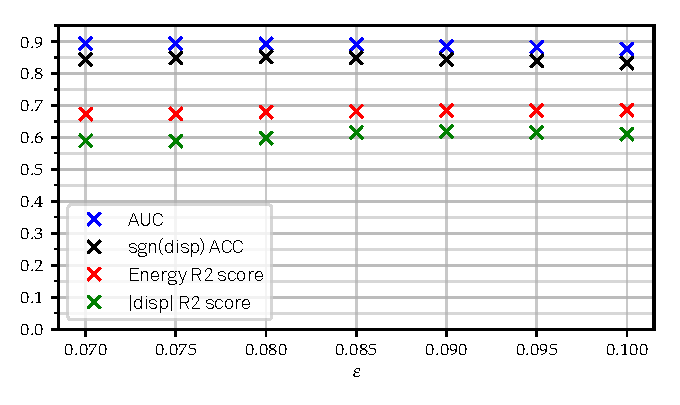
\includegraphics[width=0.85\textwidth]{Plots/Epsilon/eps_scores.pdf}
  \caption{Validation scores for the analysis tasks in dependance of the DBSCAN's $\varepsilon$. The AUC for the gamma hadron separation's ROC (blue), the source position reconstruction's accuracy of the sign(disp) (black) and the $R^2$-score for the \texttt{disp} regression (green), as well as the $R^2$-score for the energy reconstrcution (red) are shown.}
  \label{fig:eps_scores}
\end{figure}
%
\begin{figure}
  \centering
  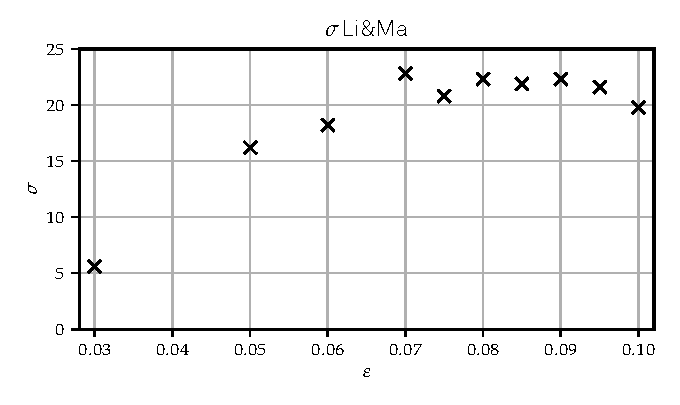
\includegraphics[width=0.85\textwidth]{Plots/Epsilon/eps_sigma.pdf}
  \caption{Detection significances for the PhotonStream open crab sample in dependancy of the DBSCAN's $\varepsilon$. The significances represent the maximum detection significance as a function of the $\theta^2$-cut and the prediction threshold of the separation.}
  \label{fig:eps_sigma}
\end{figure}
%
\begin{figure}
  \centering
  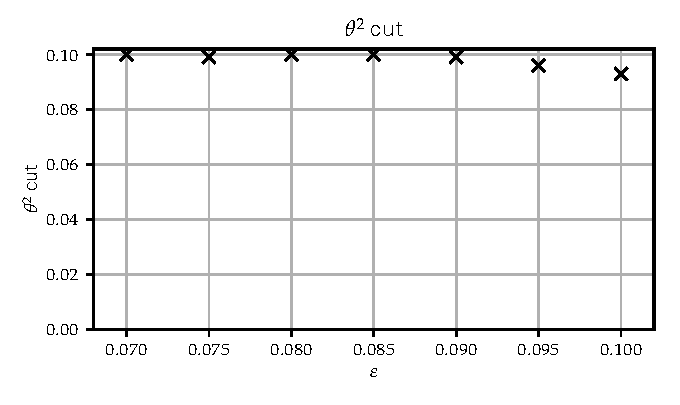
\includegraphics[width=0.85\textwidth]{Plots/Epsilon/eps_theta_cut.pdf}
  \caption{$\theta^2$ cuts for the maximum detection signifance on the PhotonStream open crab sample for different $\varepsilon$-configurations. The cuts are optimized to yield the maximum detection significance.}
  \label{fig:eps_theta}
\end{figure}

%%%%%%%%%%%%%%%%%%%%%%%%%%%%%%%%%%%%%%%%%%%%%%%%%%%%%%%%%%%%%%%%%%%%%
\section{Pixelbased Threshold Cleaning on the PhotonStream}
%%%%%%%%%%%%%%%%%%%%%%%%%%%%%%%%%%%%%%%%%%%%%%%%%%%%%%%%%%%%%%%%%%%%%
%
As shown in \autoref{fig:analysis}, the cleaning via DBSCAN is not exclusive
for PhotonStream data. The point-cloud can easily be integrated over time and
thus reprojected to the camera plane. This way the DBSCAN cleaning can be
evaluated by applying the classical pixelbased threshold cleaning, as defined
in \autoref{sec:thresh}, on PhotonStream data. Since the PhotonStream data
differs from the LP by consisting of generally brighter images (larger number
of PE), the best thresholds for air-shower pixels might differ from the ones
described in \autoref{sec:thresh}. Still, the results might explain the
differences of the novel data format.

The features of this cleaned data set resemble those of the FACT-Tools
analysis: air-showers have a rather small \texttt{length} and \texttt{width},
culminating around \num{10} rather than the large values of the DBSCAN
air-showers. Since the cleaning equals the one used within the FACT-Tools
analysis, apart from a small offset due to brighter air-showers, this is
expected. However, the data MC mismatches still remain significant, resulting
in worse performance on the analysis tasks than the DBSCAN data. The gamma-
hadron separation AUC drops to $0.7501\,\pm\,0.0019$, while the detection
significance on the data sample does not exceed $10.2\,\symup{\sigma}$. The
classification output is shown in \autoref{fig:threshg}. It becomes clear that
a large number of protons is classified as gammas by the descision trees, affecting the origin reconstruction as well. Thus,
the proton MC simulations on this cleaning look very similar to the gamma MC
simulations and the trained model is not performing well.

\begin{figure}
  \centering
  \includegraphics[width=\textwidth, page=5]{Plots/data_mc/features_thresh.pdf}
  \caption{Output of the random forest used for the gamma hadron separation on the PhotonStream data set cleaned via the pixelbased threshold method.}
  \label{fig:threshg}
\end{figure}
%
This cleaning, however, is not optimized to this data format and does not
profit from the new representation, since the point-cloud needs to be projected
back to a two-dimensional representation. Furthermore, with the PhotonStream
data containing brighter events, the thresholds might be to low and background
pixels may survive the cleaning. However, even with higher cleaning thresholds,
it appears that the DBSCAN cleaning is way better suited for the PhotonStream
data format and there is, indeed, quite some optimization needed to find the
right analysis parameters for this new data format.
